\documentclass[border=5pt]{standalone}
\usepackage{tikz}
\usepackage{amsmath}
\usetikzlibrary{calc, positioning, arrows.meta, 3d}
\begin{document}
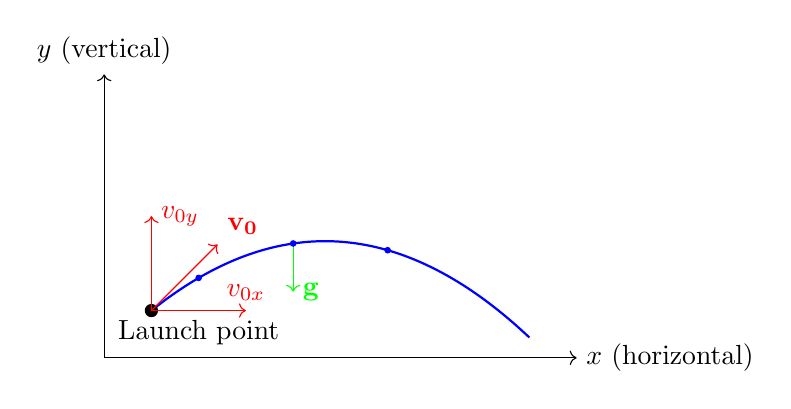
\begin{tikzpicture}[scale=1.2]
% Draw axes
\draw[->] (0,0) -- (5,0) node[right] {$x$ (horizontal)};
\draw[->] (0,0) -- (0,3) node[above] {$y$ (vertical)};

% Draw trajectory
\draw[thick, blue] plot[smooth,domain=0.5:4.5] (\x, {0.5 + 1.2*(\x-0.5)/1.5 - 4.9*(\x-0.5)^2/(1.5^2*10)});

% Mark launch point
\fill (0.5,0.5) circle (2pt);
\node[below] at (1,0.5) {Launch point};

% Draw initial velocity components
\draw[red, ->] (0.5,0.5) -- (1.5,0.5) node[above] {$v_{0x}$};
\draw[red, ->] (0.5,0.5) -- (0.5,1.5) node[right] {$v_{0y}$};
\draw[red, ->] (0.5,0.5) -- (1.2,1.2) node[above right] {$\mathbf{v_0}$};

% Draw gravity
\draw[green, ->] (2,1.2) -- (2,0.7) node[right] {$\mathbf{g}$};

% Mark some points on trajectory
\foreach \x in {1,2,3} {
    \fill[blue] (\x, {0.5 + 1.2*(\x-0.5)/1.5 - 4.9*(\x-0.5)^2/(1.5^2*10)}) circle (1pt);
}
\end{tikzpicture}
\end{document}
